% begin module horizontal-tangent-ex4
\begin{frame}
\begin{example}[Example 4, p. 138]
\begin{columns}[c]
\column{.35\textwidth}
\ \only<handout:0| -7>{%
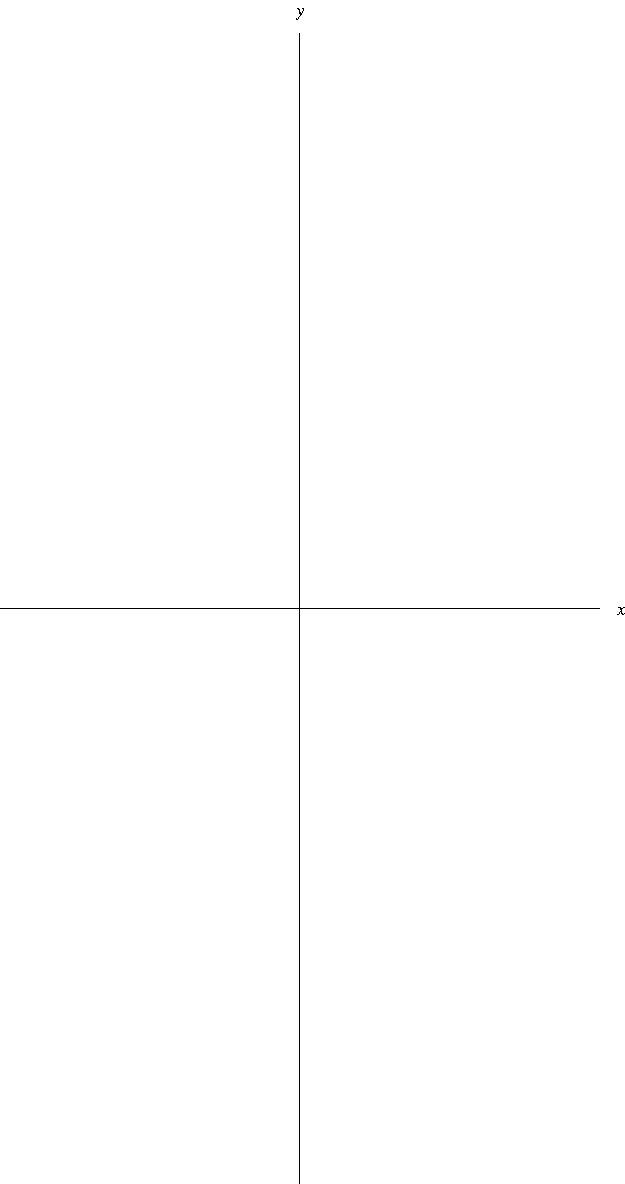
\includegraphics[height=7cm]{derivatives/pictures/03-03-ex4a.pdf}%
}%
\only<8->{%
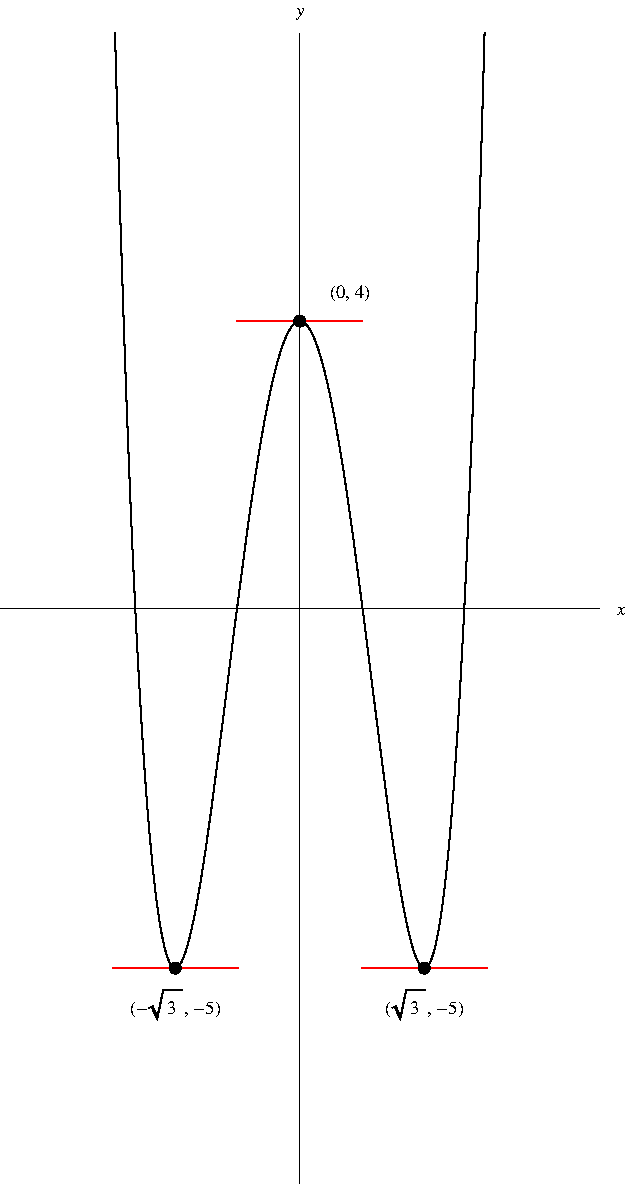
\includegraphics[height=7cm]{derivatives/pictures/03-03-ex4b.pdf}%
}%
\column{.65\textwidth}
Find the points on the curve $y = x^4 - 6x^2 + 4$ where the tangent line is horizontal.
%\abovedisplayskip=0pt
%\belowdisplayskip=0pt
\begin{eqnarray*}
\uncover<2->{\frac{\diff y}{\diff x}} & \uncover<2->{ = } & %
\uncover<3->{\frac{\diff}{\diff x}(x^4) - 6\frac{\diff}{\diff x}(x^2) + \frac{\diff}{\diff x}(4)}\\
& \uncover<4->{ = } & %
\uncover<4->{4x^3 - 12x + 0} \uncover<5->{ = 4x(x^2-3)}
\end{eqnarray*}
\begin{itemize}
\item<6->  Horizontal tangents occur where the derivative is 0.
\item<7->  $\frac{\diff y}{\diff x} = 0$ if $x = 0$ or $x^2 - 3 = 0$, that is, $x = \pm \sqrt{3}$.
\item<8->  Points: $(0,4), (-\sqrt{3},-5), (\sqrt{3},-5)$.
\end{itemize}
\end{columns}
\end{example}
\end{frame}
% end module horizontal-tangent-ex4
